\section{Experimental Setup}

\begin{figure}[H]
\begin{center}
  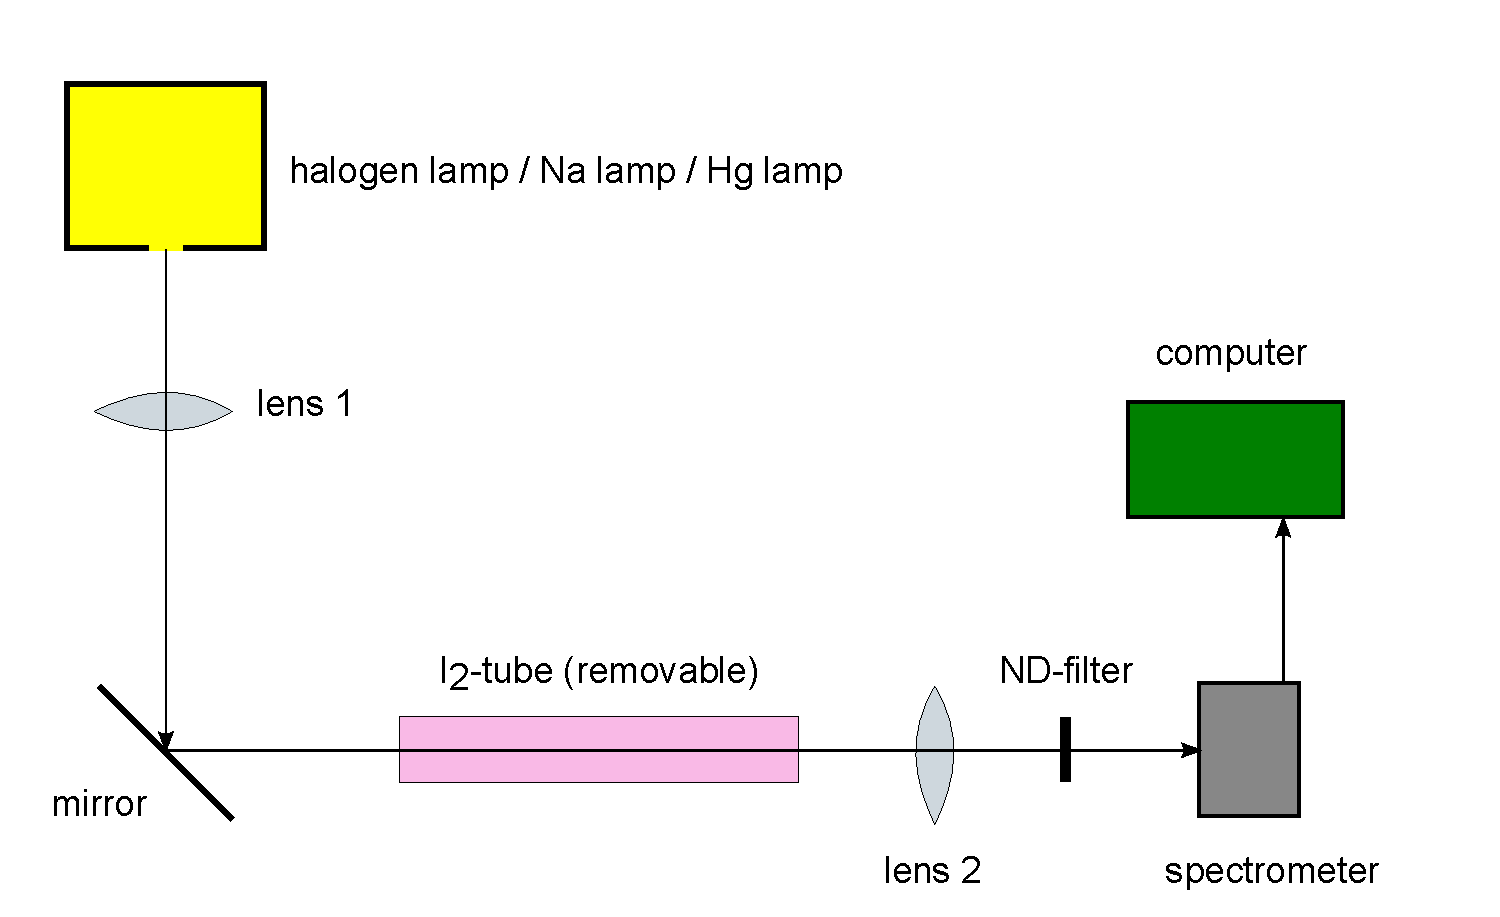
\includegraphics[width=\textwidth]{../img/aufbau.pdf}
  \caption[---]{Experimental setup for measuring the emission spectra of different lamps and
  the transmission spectrum of I$_2$.}
  \label{img:aufbau}
\end{center}
\end{figure}

\autoref{img:aufbau} shows the experimental setup which has been constructed on an optical bench.
As a light source, two lamps with discrete spectra (Na and Hg lamp) or a
halogen lamp with continuous spectrum can be mounted.
The light from the lamp is collimated by lens 1 and then reflected by 90$^{\circ}$ with a mirror.
To measure the absorption of I$_2$, a glass tube filled with grains of solid iodide can be inserted in the
optical path.
Before the light enters the spectrometer, it is focused with lens 2 and its intensity
reduced with a exchangeable neutral density filter.
The data from the spectrometer \emph{ocean optics USB2000+} is then captured on a computer.
